\section{The ARM7TDMI Microprocessor Simulator Description}

The ARM7TDMI core is a member of the ARM family of general-purpose 32-bit microprocessors.
The ARM family offers high performance for very low power consumption, and small size.

The ARM7TDMI architecture is based on \emph{Reduced Instruction Set Computer} (RISC) principles.
It uses a three-stage pipeline, so instructions are executed in three stages:
\begin{itemize}
	\item Fetch: instruction fetched from memory.
	\item Decode: decoding of registers used in instruction.
	\item Execute: register(s) read from register bank, shift and/or ALU operation, write register(s) back to register bank.
\end{itemize}
A total of 32 registers are available.
However, the processor has seven modes of execution, and while executing in a given mode the processor has only access to a subset (concretely sixteen registers) of them.
Additionally, the ARM7TDMI can execute two different instruction sets (ISAs):
\begin{itemize}
	\item Standard ARM ISA: it is composed of 32 bits RISC instructions. This is the main ISA of the ARM processors series.
	\item Thumb ISA: it is composed of 16 bits RISC instructions. This ISA is used to reduce code footprint, however the number of instructions proposed by this ISA is reduced, so not all kind of operations can done using this ISA.
\end{itemize}
The two ISAs are fully supported by the simulator.

For the development of the ARM7TDMI simulator developed at CEA LIST the following documents were used:
\begin{itemize}
	\item ARM Architecture Reference Manual
	\item ARM7TDMI (Rev 4) Technical Reference Manual
\end{itemize}
Please refer to them if you are looking for more details on the ARM7TDMI processor.

\begin{figure}[!h]
	\begin{center}
		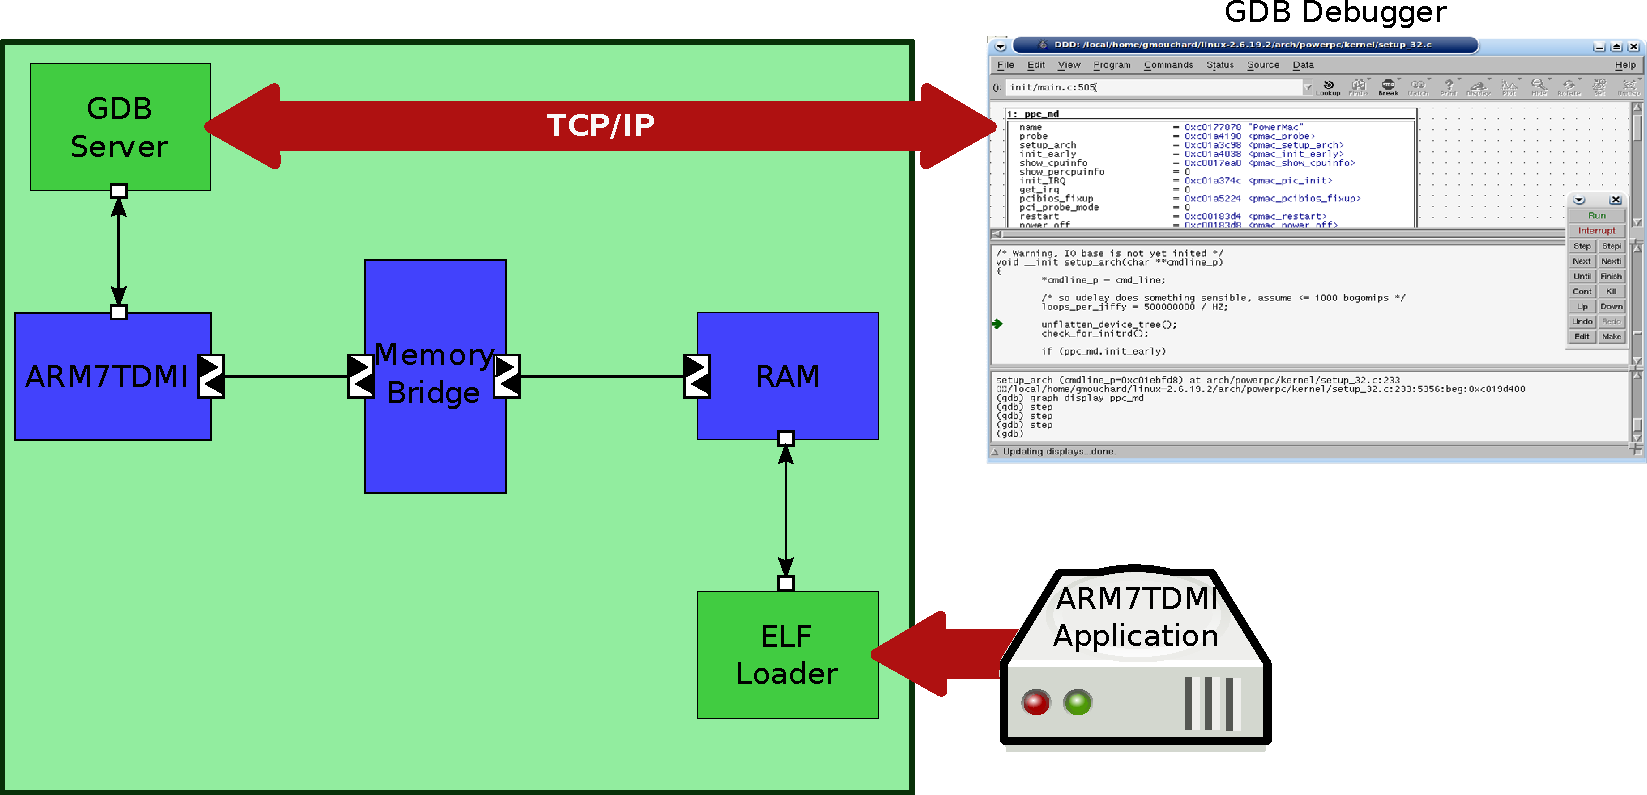
\includegraphics[width=\textwidth]{figures/ARM7TDMI_architecture.pdf}
	\end{center}
	\caption{ARM7TDMI schematic architecture.}
	\label{fig:arm7tdmi_architecture}
\end{figure}

Figure~\ref{fig:arm7tdmi_architecture} shows the schematic architecture of the simulator used for the validation of the ARM7TDMI processor.
The simulator itself consist on three components (the blue boxes on Figure~\ref{fig:arm7tdmi_architecture}):
\begin{itemize}
	\item \textbf{ARM7TDMI:} this component models the ARM7TDMI processor itself.
	\item \textbf{Memory Bridge:} this component allows the connection of the ARM7TDMI processor to the main memory.
	\item \textbf{RAM:} this component is the memory of the system. The processor uses it to load the program to run and store temporary information.
\end{itemize}

Additionally, the simulator provides two services (green boxes on Figure~\ref{fig:arm7tdmi_architecture}):
\begin{itemize}
	\item \textbf{ELF Loader:} thanks to this service ARM7TDMI binaries can be loaded into the RAM component.
	\item \textbf{GDB Server:} this service enables extended debugging with the help of an external client debugger, as for example: gdb, ddd, eclipse debugger, and others.
\end{itemize}
